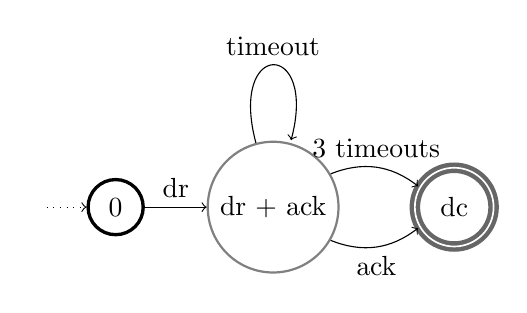
\begin{tikzpicture}
[
init/.style={circle, draw=black!100, very thick, minimum size=7mm,node distance=2cm},
state_split/.style={circle split, draw=gray!100, thick, minimum size=7mm,node distance=2cm},
state/.style={circle, draw=gray!100, thick, minimum size=7mm,node distance=2cm},
final/.style={circle,double, draw=black!60,  ultra thick, minimum size=10mm,node distance=23mm}
]
%Nodes
\node[init]         (start)                         {0};
\node               (em)        [left of=start]     {};
\node[state]        (send_dr)   [right of=start]    {dr + ack};
\node[final]        (dc_ack)    [right of=send_dr]  {dc};


%Lines
%\draw[->] (start.east) -- (synx.west);
%\draw[->] (synx.east) -- (end.west);
%\path[->] (start)  edge [loop above] node {a} (start); 
\draw[dotted, ->] (em.east) -- (start.west);
\path[->] 
(start)   edge                   node [above]   {dr}    (send_dr)
(send_dr) edge [bend left]       node [above]   {3 timeouts} (dc_ack)
(send_dr) edge [bend right]      node [below]   {ack}     (dc_ack)
(send_dr) edge [loop above]      node           {timeout}   (send_dr);
\end{tikzpicture}